\chapter{Introduction}
Everyone has probably had the experience of walking into a restaurant which has a menu that makes no sense and not knowing what to expect would then ask the waiter to recommend some quality dishes that are native to the restaurant. The waiter would then go on to list some of the specialities of the restaurant, some favorites of other customers and to some extent also explain the  meat or flavoring that the dish comprises of. Finally, the customer would then make a decision on what would be appropriate to his own tastes.

Recommender systems are no less different from the waiter of that unfamiliar restaurant. They strive to satisfy the user's needs by providing a quality experience taking his own tastes and interests into account. The core aspect of a recommender is to not pose a user with too much information but only give him what he desires. Recommender systems heavily rely upon user feedback as a form of learning user behaviour and interests. Conventional recommender systems make use of explicit user ratings on items and where ratings are not available, they make use of clicks. For further personalization, clicks are often enriched with meta-data regarding the item, for instance tags. In addition, many web applications do not make use of an explicit `dislike' button as this is often conceived as offending the original author of the item. While there exists a `like' button which in most cases implicates a good recommendation was received, there is no direct way to capture the opposite.

Various forms of meta-data have been extensively studied as forms of user feedback. Ye et al. investigate geo-location awareness enriched upon social networking for recommending new locations \cite{ye_location_2010}.  Castagnos et al. report implications of eye tracking for recommendation in an e-commerce scenario \cite{castagnos_eye-tracking_2010}. Liu et al. move further into the user's body by investigating user's heartbeat as an attribute towards personalized music recommendation \cite{liu_music_2009}. While the rate at which sensors evolve over the years, it is inevitable that this would be the future of recommendations. But, there is a more personal and explicit form of feedback that has been ignored all along. 

Consider the case of a cold state scenario where a new user probes the system and clicks on one of the top recommendations and the user did not like want was presented in the item either because the original title to the item was misleading or he had accidentally clicked on it. In a naive click based recommendation, the user is immediately flooded with similar items. As most web applications often tie the hands of users by not providing explicit `dislike' feedback, they then turn to the only possible way of expressing 
their discontent - comments.

Comments have evolved over the years, initially it was perceived as a form of providing feedback. Now, with introduction of various features such as `upvote/downvote' comments have now become more of a struggle to achieve the most votes through witty opinions or providing genuine additive information. The `reply' feature in comments have also turned commenting platforms into conversational mediums leading to heated debates. In this work, we perform exploratory research into discovering the usefulness of this unique user feedback medium towards personalization in recommendations.

\newpage
\section{Research Flow}
Over the course of our work, we will answer the following research questions. Figure~\ref{fig:r_questions_rep} in essence represents what factors to take into consideration while training the model for our recommender, whereas Figure~\ref{fig:r_questions_pred} represents that of making predictions using our model. Finally, Figure~\ref{fig:r_questions_misc} refers to domain specific questions as we are investigating the particular domain of news recommendation.

\begin{figure}[!h]
\centering
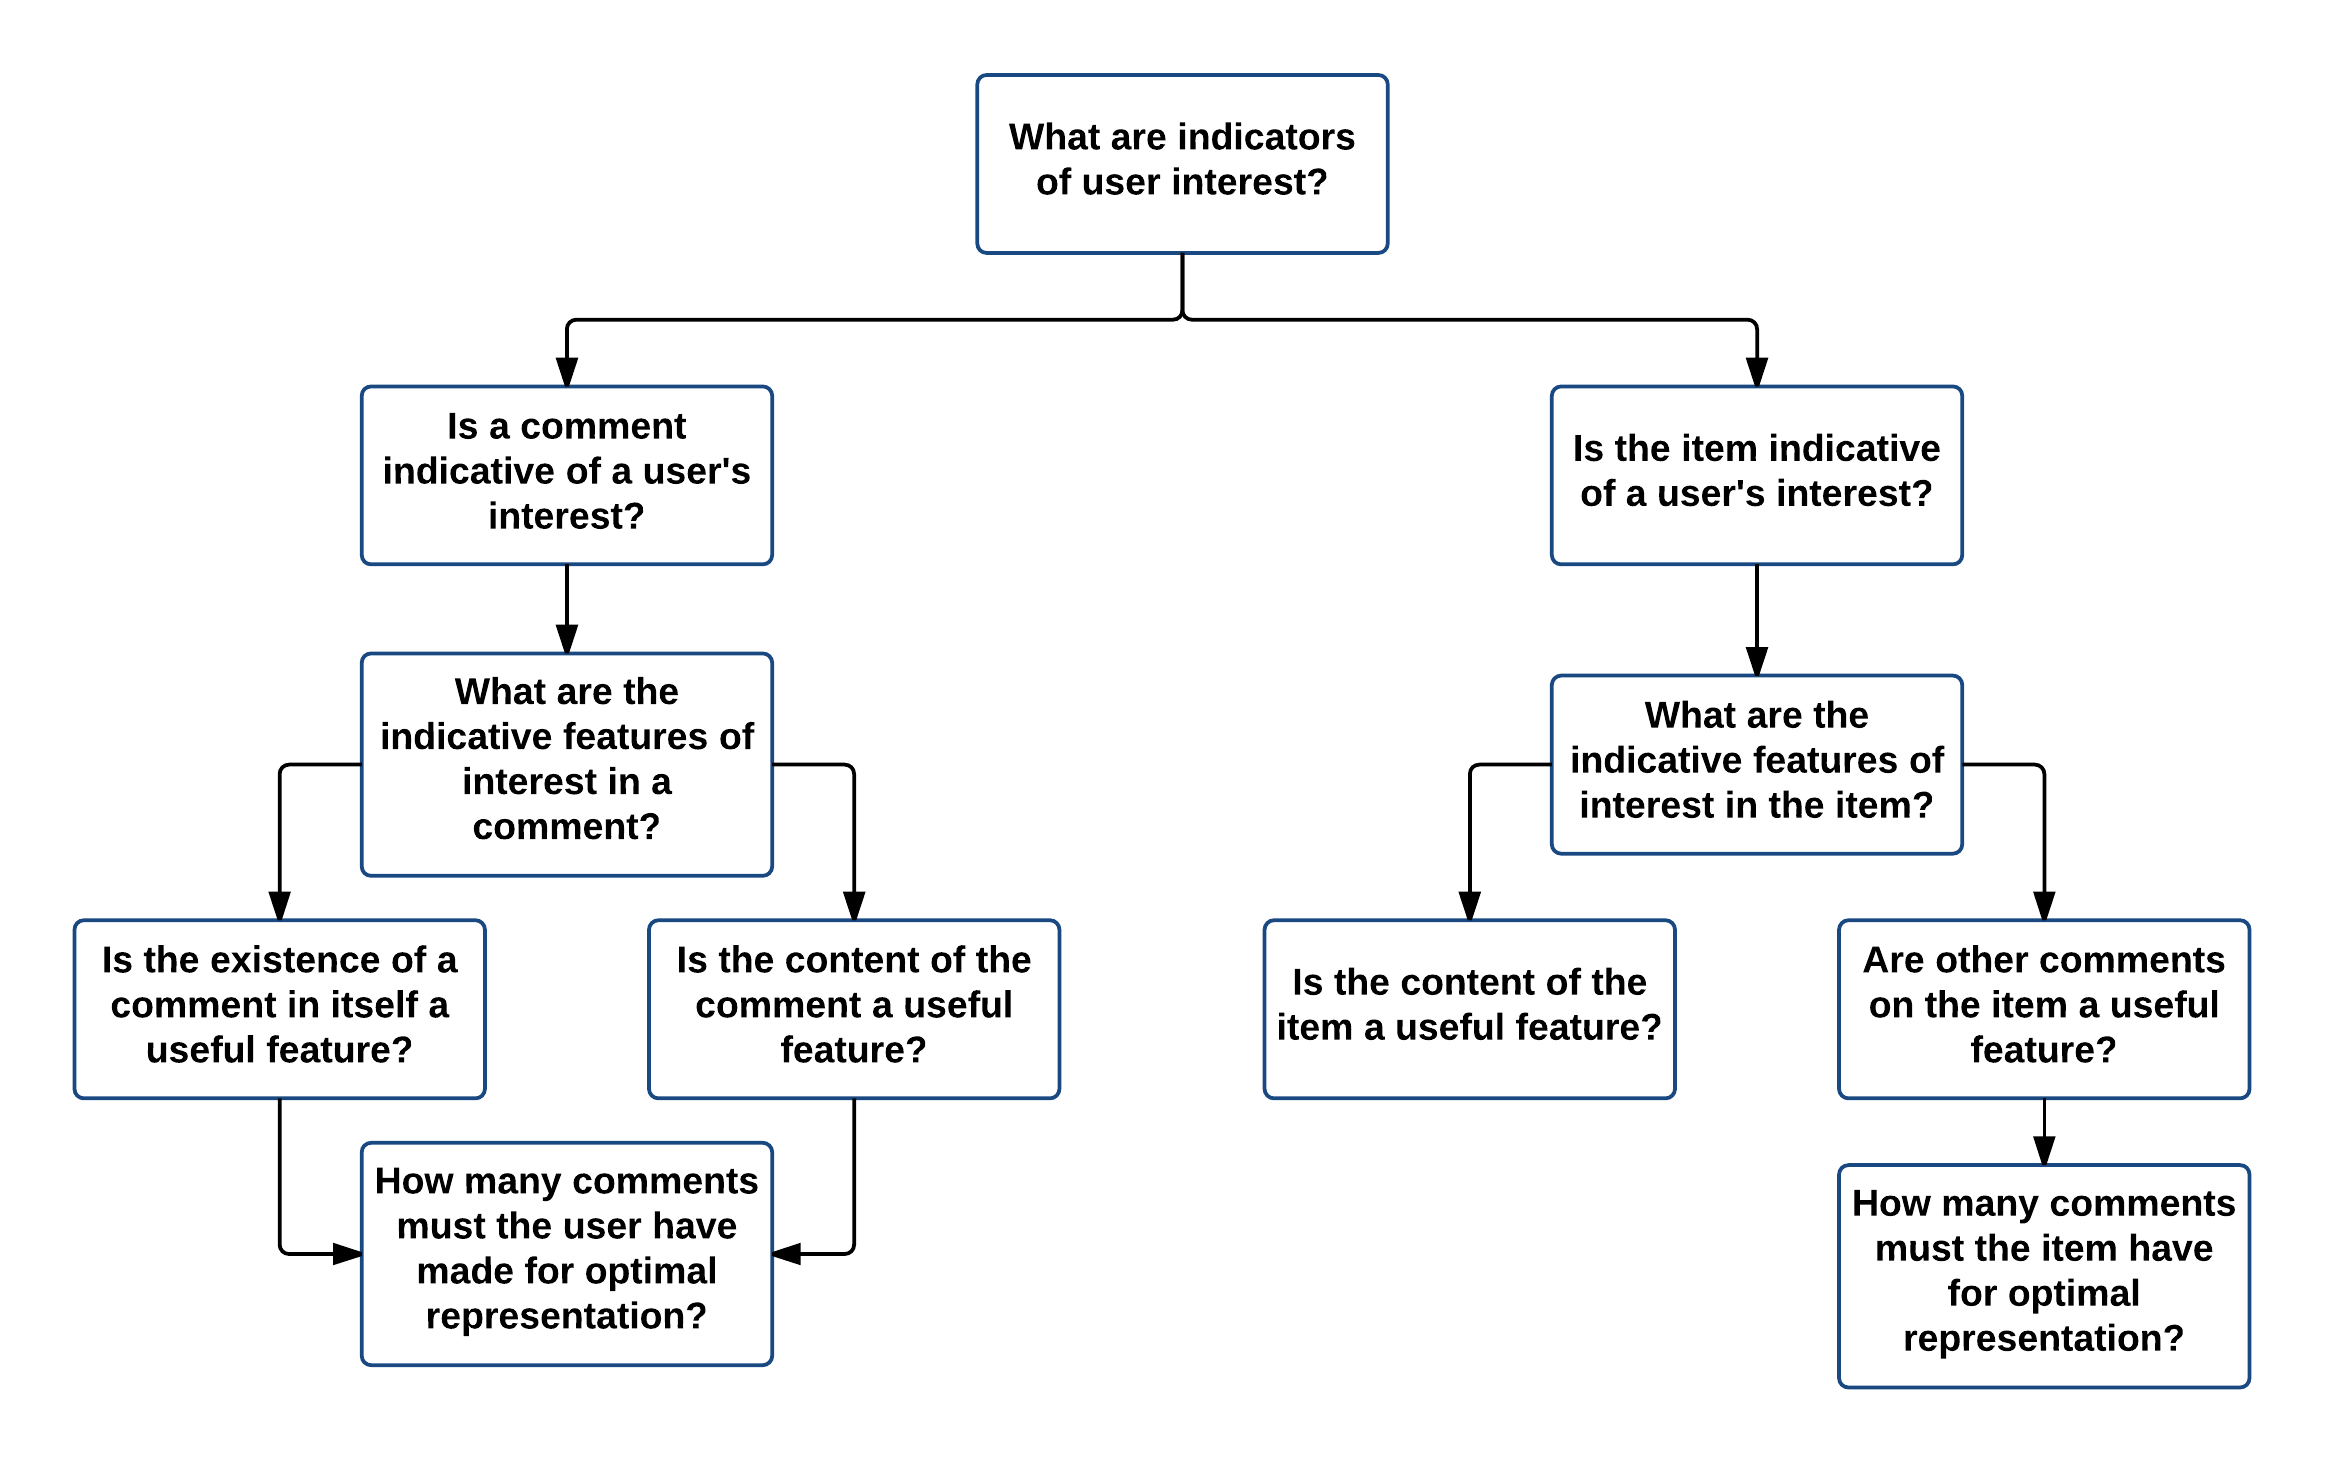
\includegraphics[width=0.905\textwidth]{c-intro_images/r_questions_1.png}
\caption{Representation of Interest}
\label{fig:r_questions_rep}
\end{figure}

\begin{figure}[!h]
\centering
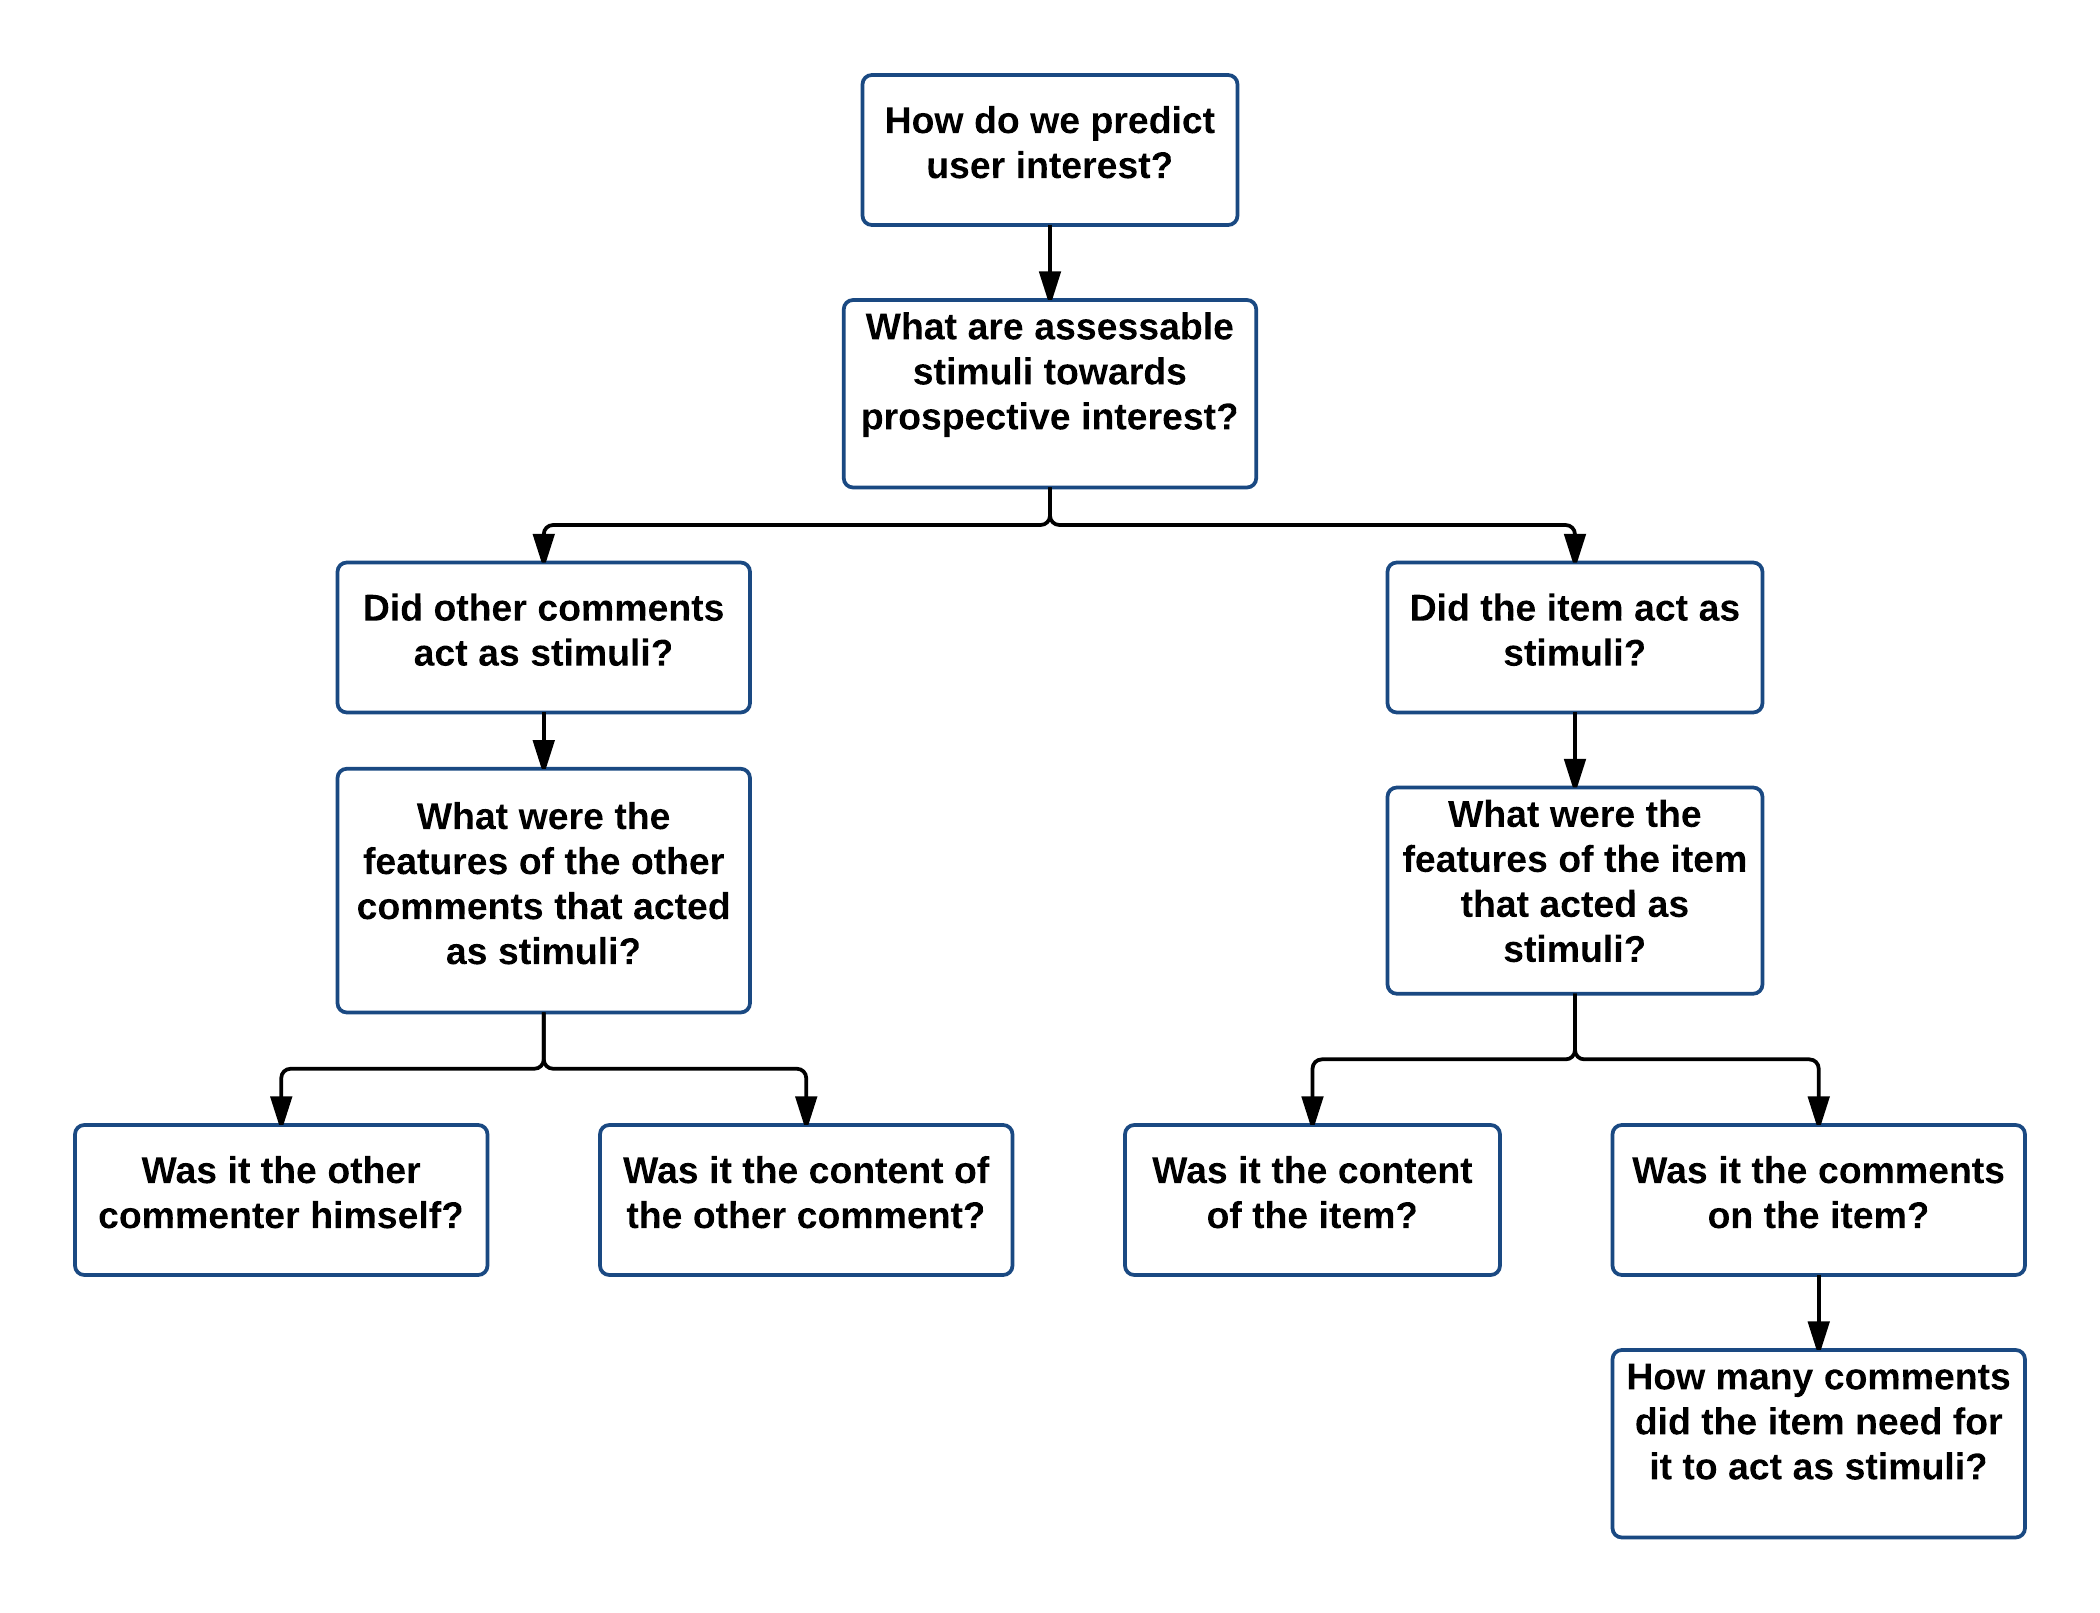
\includegraphics[width=0.8\textwidth]{c-intro_images/r_questions_2.png}
\caption{Prediction of Interest}
\label{fig:r_questions_pred}
\end{figure}

\begin{figure}[!h]
\centering
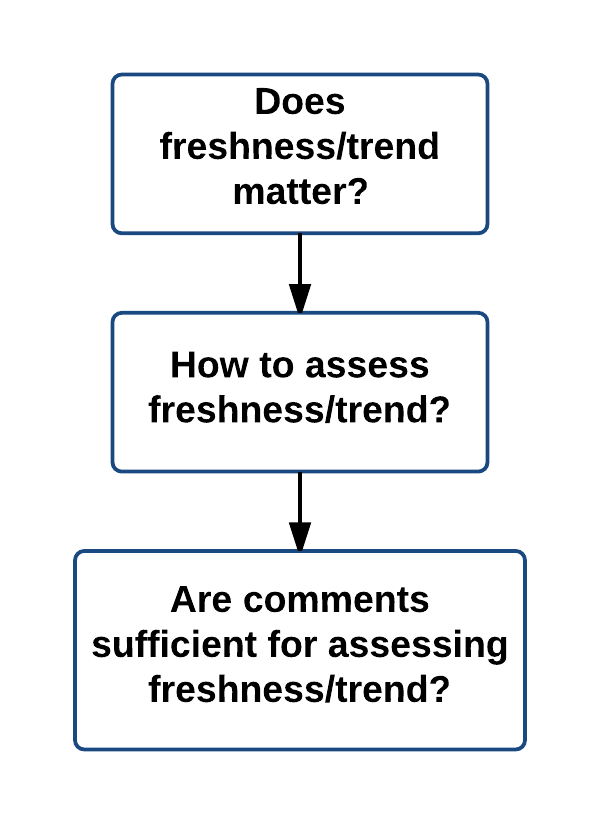
\includegraphics[width=0.25\textwidth]{c-intro_images/r_questions_3.png}
\caption{Domain Specific}
\label{fig:r_questions_misc}
\end{figure}

\section{Thesis Organization? (TODO)}